\documentclass[border=6pt]{standalone}
\usepackage{tikz}
\usepackage{amsmath}
\usetikzlibrary{fit,positioning}
\begin{document}
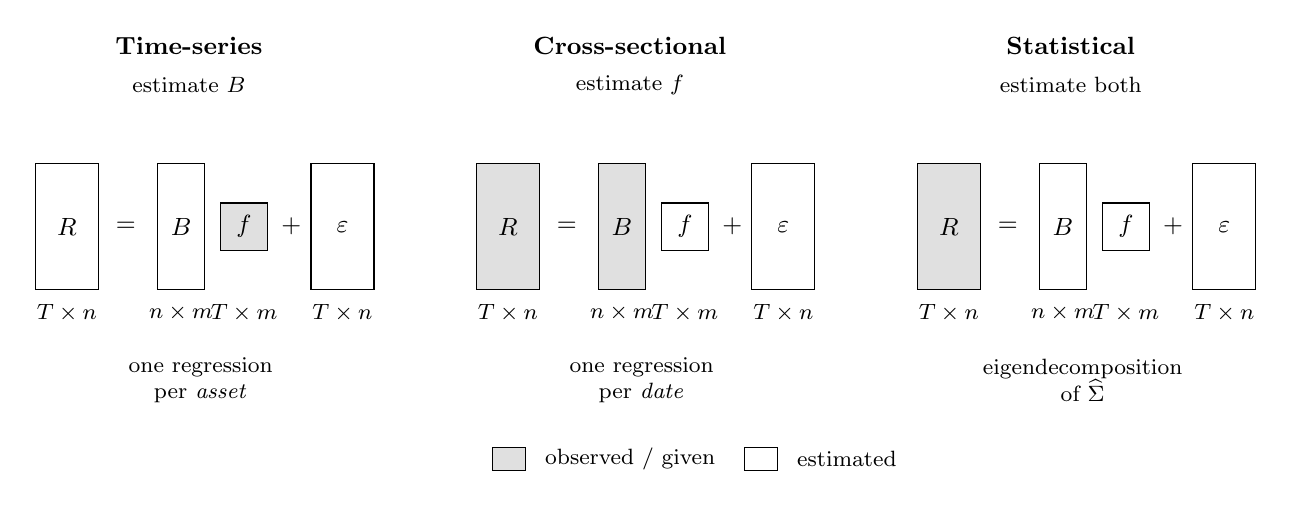
\begin{tikzpicture}[font=\small,
  known/.style={draw,fill=black!12,minimum height=#1,minimum width=8mm},
  unk/.style={draw,fill=white,minimum height=#1,minimum width=8mm},
  lbl/.style={font=\footnotesize},
  ttl/.style={font=\small\bfseries}]

% ---------- panel 1 : time series ----------
\begin{scope}[xshift=0cm]
  \node[ttl] at (1.55,3.5) {Time-series};
  \node[lbl,align=center] at (1.55,3.0) {estimate $B$};
  \node[unk=16mm]  (R1) at (0,1.2) {$R$};
  \node at (0.75,1.2) {$=$};
  \node[unk=16mm,minimum width=6mm] (B1) at (1.45,1.2) {$B$};
  \node[known=6mm,minimum width=6mm] (F1) at (2.25,1.2) {$f$};
  \node at (2.85,1.2) {$+$};
  \node[unk=16mm] (E1) at (3.5,1.2) {$\varepsilon$};
  \node[lbl] at (0,0.1) {$T\times n$};
  \node[lbl] at (1.45,0.1) {$n\times m$};
  \node[lbl] at (2.25,0.1) {$T\times m$};
  \node[lbl] at (3.5,0.1) {$T\times n$};
  \node[lbl,align=center] at (1.7,-0.75) {one regression\\per \emph{asset}};
\end{scope}

% ---------- panel 2 : cross sectional ----------
\begin{scope}[xshift=5.6cm]
  \node[ttl] at (1.55,3.5) {Cross-sectional};
  \node[lbl,align=center] at (1.55,3.0) {estimate $f$};
  \node[known=16mm] (R2) at (0,1.2) {$R$};
  \node at (0.75,1.2) {$=$};
  \node[known=16mm,minimum width=6mm] (B2) at (1.45,1.2) {$B$};
  \node[unk=6mm,minimum width=6mm] (F2) at (2.25,1.2) {$f$};
  \node at (2.85,1.2) {$+$};
  \node[unk=16mm] (E2) at (3.5,1.2) {$\varepsilon$};
  \node[lbl] at (0,0.1) {$T\times n$};
  \node[lbl] at (1.45,0.1) {$n\times m$};
  \node[lbl] at (2.25,0.1) {$T\times m$};
  \node[lbl] at (3.5,0.1) {$T\times n$};
  \node[lbl,align=center] at (1.7,-0.75) {one regression\\per \emph{date}};
\end{scope}

% ---------- panel 3 : statistical ----------
\begin{scope}[xshift=11.2cm]
  \node[ttl] at (1.55,3.5) {Statistical};
  \node[lbl,align=center] at (1.55,3.0) {estimate both};
  \node[known=16mm] (R3) at (0,1.2) {$R$};
  \node at (0.75,1.2) {$=$};
  \node[unk=16mm,minimum width=6mm] (B3) at (1.45,1.2) {$B$};
  \node[unk=6mm,minimum width=6mm] (F3) at (2.25,1.2) {$f$};
  \node at (2.85,1.2) {$+$};
  \node[unk=16mm] (E3) at (3.5,1.2) {$\varepsilon$};
  \node[lbl] at (0,0.1) {$T\times n$};
  \node[lbl] at (1.45,0.1) {$n\times m$};
  \node[lbl] at (2.25,0.1) {$T\times m$};
  \node[lbl] at (3.5,0.1) {$T\times n$};
  \node[lbl,align=center] at (1.7,-0.75) {eigendecomposition\\of $\widehat{\Sigma}$};
\end{scope}

% legend
\draw[draw,fill=black!12] (5.4,-1.9) rectangle ++(0.42,0.30);
\node[lbl,anchor=west] at (5.95,-1.75) {observed / given};
\draw[draw,fill=white] (8.6,-1.9) rectangle ++(0.42,0.30);
\node[lbl,anchor=west] at (9.15,-1.75) {estimated};
\end{tikzpicture}
\end{document}
